\documentclass[a4paper, DIV=13]{scrartcl}

\usepackage[
typ=ib,
fach=Mathematik,
lerngruppe=2BF,
farbig,
namensfeldAnzeigen,
datumAnzeigen,
seitenzahlen = auto,
loesungen = seite,
module= {Papiertypen}
]{schule}


\usepackage{amsmath}
\usepackage{float}
\usepackage[]{fourier-otf}
\usepackage{microtype}	
\author{Maximilian Hertenstein}
\date{\today}
\title{Geradengleichungen bestimmen}
\date{Datum: \hspace{1.5cm}}

\usepackage{tkz-base}
\usepackage{tkz-fct}
\usepackage{tkz-euclide}
\ifoot{% TODO: \usepackage{graphicx} required

		
\includegraphics[width=0.3\linewidth]{GHSE-Logo}

}

\begin{document}

Manchmal muss man beim Bestimmen der Steigung mehrere Einheiten nach rechts gehen, um einen weiteren Punkt auf der Geraden und gleichzeitig eine Ecke des Koordinatensystems zu erreichen.

Die Steigung ist dann:

$$
m=\frac{\text{Entfernung in y-Richtung}}{\text{Entfernung in x-Richtung}}
$$



\vskip 20pt


\begin{minipage}{0.5\linewidth}

\begin{center}
		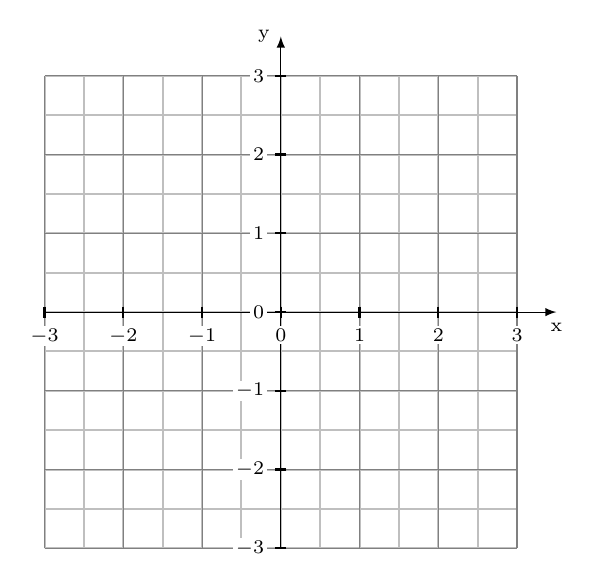
\begin{tikzpicture}[scale = 1]
			\scriptsize
			\tkzInit[ymax=3, xmax=3, xmin=-3, ymin = -3,xstep=1,ystep=1]
			\tkzGrid[sub,subxstep=0.5, subystep=0.5]
			\tkzFct[samples=50,domain=-5:5]{-0.5*x +2}
			%\tkzSetUpAxis[line width=10pt,tickwd=0pt,ticka=0pt,tickb=0pt]
			\tkzAxeXY[/tkzdrawX/label=x,/tkzdrawY/label=y]
			
		\end{tikzpicture}

		
	\end{center}
\end{minipage}
\begin{minipage}{0.5\linewidth}

\begin{center}
		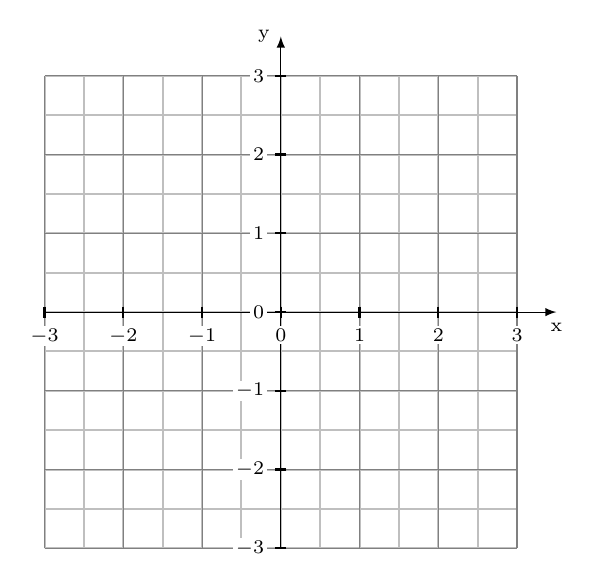
\begin{tikzpicture}[scale = 1]
			\scriptsize
			\tkzInit[ymax=3, xmax=3, xmin=-3, ymin = -3,xstep=1,ystep=1]
			\tkzGrid[sub,subxstep=0.5, subystep=0.5]
			\tkzFct[samples=50,domain=-5:5]{(0.66666666666)*x - 1}
			%\tkzSetUpAxis[line width=10pt,tickwd=0pt,ticka=0pt,tickb=0pt]
			\tkzAxeXY[/tkzdrawX/label=x,/tkzdrawY/label=y]
			
		\end{tikzpicture}

		
	\end{center}
\end{minipage}



\begin{minipage}{0.5\linewidth}
\begin{align*}
m=& \\
b=& \\
f\colon y=
\end{align*}
\begin{center}
\begin{tabular}{|c|c|c|c|}
\hline
x & $-2$ & $0$ & $2$  \\
\hline
y &\qquad & \qquad & \qquad  \\
\hline
\end{tabular}
\end{center}

\end{minipage}
\begin{minipage}{0.5\linewidth}
\begin{align*}
m=& \\
b=& \\
f\colon y=
\end{align*}
\begin{center}
\begin{tabular}{|c|c|c|c|}
\hline
x & $-3$ & $0$ & $3$  \\
\hline
y &\qquad & \qquad & \qquad  \\
\hline
\end{tabular}
\end{center}
\end{minipage}

\section{Regel}

		Die Steigung einer Geraden durch zwei Punkte $P(x_P \mid y_P)$ und $Q(x_Q \mid y_Q)$ lässt sich mit der Formel $$m= \dfrac{{y_Q-y_P}}{{x_Q-x_P}}$$ bestimmen.


\begin{figure}[H]
	\begin{center}
		
		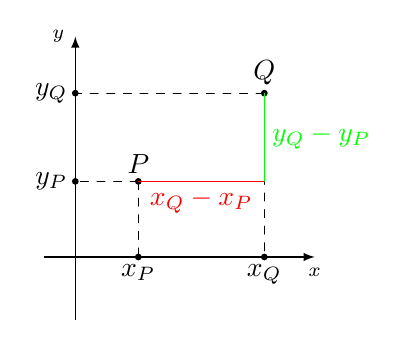
\begin{tikzpicture}[scale = .8]
			\scriptsize
			\tkzInit[ymax=3, xmax=3.3, xmin=-0.5, ymin = -1,xstep=1,ystep=1]
			
			
			%\tkzSetUpAxis[line width=10pt,tickwd=0pt,ticka=0pt,tickb=0pt]
				\tkzDrawX[label=$x$,noticks]
			\tkzDrawY[label=$y$,noticks]
			\tkzFct{0.7* x + 0.5}
			\tkzDefPoints{1/1.2/P, 3/2.6/Q, 1/0/Px, 0/1.2/Py, 3/0/Qx, 0/2.6/Qy, 3/1.2/C}
			
			\tkzDrawPoints[](P,Q, Px, Py, Qx, Qy)
	\tkzLabelPoint[above](P){$P$}
	\tkzLabelPoint[above](Q){$Q$}
	\tkzLabelPoint[](Px){$x_P$}
	\tkzLabelPoint[](Qx){$x_Q$}
	\tkzLabelPoint[left](Py){$y_P$}
	\tkzLabelPoint[left](Qy){$y_Q$}
	\tkzDrawSegment[dashed](P,Px)
		\tkzDrawSegment[dashed](P,Py)
		\tkzDrawSegment[dashed](Q,Qx)
			\tkzDrawSegment[dashed](Q,Qy)
			
	\tkzDrawSegment[red](P,C)
	\tkzLabelSegment[red](P,C){$x_Q-x_P$}
		\tkzDrawSegment[green](Q,C)
			\tkzLabelSegment[right, green](Q,C){$y_Q-y_P$}
%			\tkzDrawLine[thick, add=0.5 and 0.35](P,Q)
%			\tkzDrawSegment[thick, red](P,C)
%			\tkzDrawPoints[](P,Q)
%			\tkzLabelPoints[above](P,Q)
%			\tkzDrawSegment[thick, green](Q,C)
		\end{tikzpicture}
	\end{center}
\end{figure}

\end{document} 